\documentclass[../../../main]{subfiles}


\newcommand{\incfig}[1]{%
    \def\svgwidth{\columnwidth}
    \import{./figures/}{#1.pdf_tex}
}
\begin{document}

\section*{Microcontroller implementation}

This section as the purpose of detailing how the software for the Tiva microcontroller is setup and why. The responsibility of the Tiva is to act as the brain of the entire system while the FPGA acts like a data acquisitions device and a hardware controller. 

The operating system used as the platform on the Tiva is FreeRTOS, an open source RealTime operating system created by Real Time Engineers LTD.

FreeRTOS handles multiple different types of work by dividing it into user defined tasks that are the run using a preemptive scheduler which allows the system to not only run multiple tasks in "parallel" but also efficiently allocate the resources available.


A task is a single area of responsibility that either by necessity or by convention is combined as single unit. Each task in the system (a full overview can be seen in the task diagram) can then be scheduled based on the priority is has been assigned and whether it has any meaningful work to do. 


\section*{Scheduling}

In order to enable the microcontroller to run more then one task some form of scheduling must be implemented. This allows the operating system to make a choice as to what task needs processing capacity at this moment in time. In the FreeRTOS based system running on the Tiva scheduling is done trough a priority based preemption capable implementation.

The preemption capability enables the system to respond quickly to higher priority tasks becoming available for execution rather then waiting for the current task to finish on its on, it will be paused and the higher priority task executed before the lower priority one is resumed and potentially completed.


\begin{itemize}
    \item Priority
    \item Preemption
    \item Process
\end{itemize}

\section*{Inter-task communication}

\begin{itemize}
    \item Queues
    \item State Buffers
\end{itemize}









\begin{figure}[H]
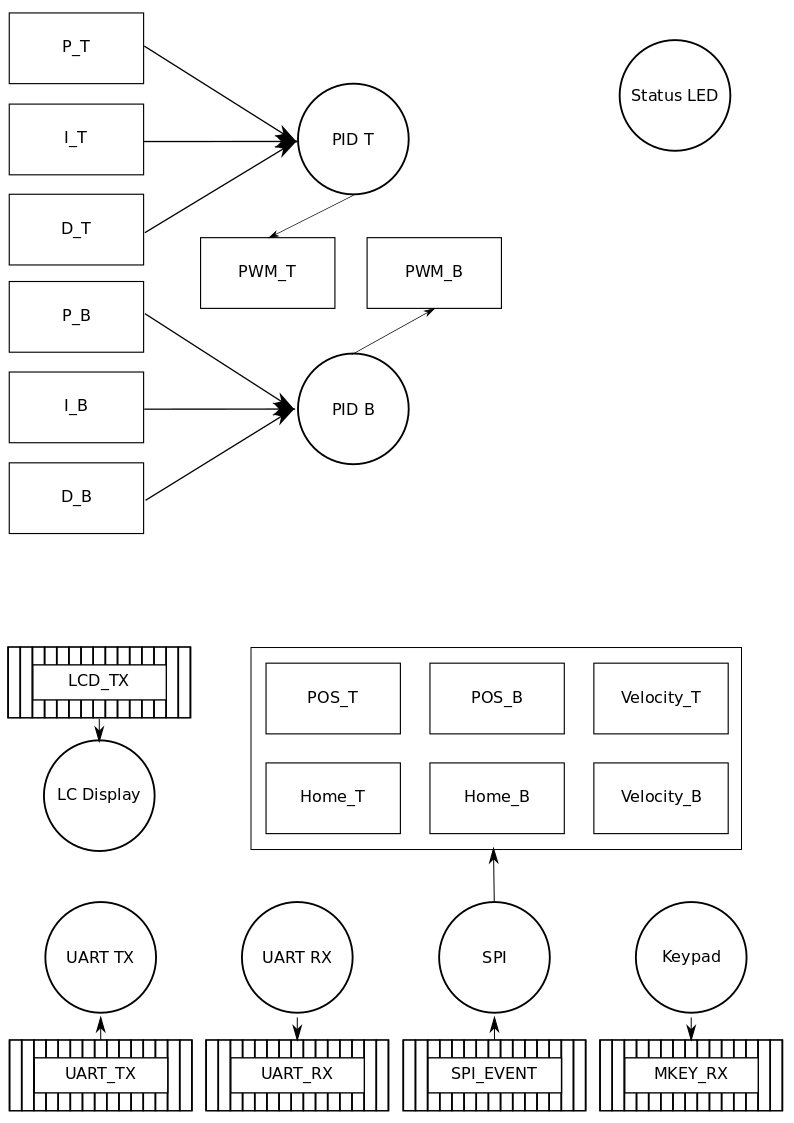
\includegraphics[width=\columnwidth]{taskdiagram_full.png}
\end{figure}
\end{document}

